\chapter{Charge transfer in amorphous systems}
\label{chap:surface_hopping_app}
Although it is important to know the maximum bound on the mobility of the charge carrier in a perfect crystal of an organic semiconductor, in reality it is very difficult to control defect formation in OSs\cite{NGUYEN2006198i, Ray2014}. This is due to van der Waals forces only weakly holding molecules at lattice sites, allowing molecules greater freedom than in traditional inorganic crystal, and increasing the chance of defect formation which can trap/scatter charge carriers reducing overall mobility. This means it is important to investigate and characterise charge transport properties for not just perfectly crystalline OSs but also those that show a range of amorphicity.
\\
\begin{wrapfigure}{r}{0.4\textwidth}
	\vspace*{-0.5cm}
	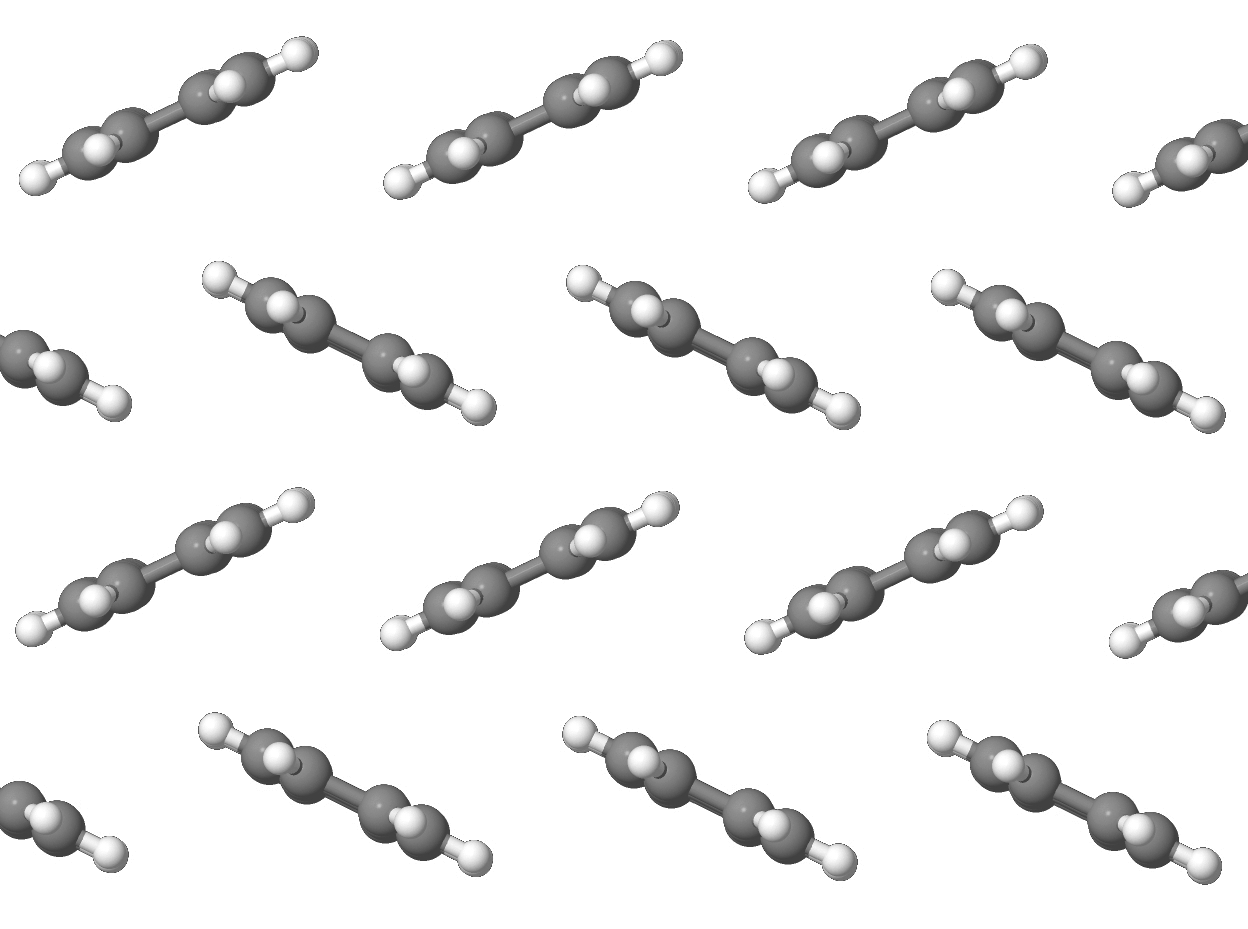
\includegraphics[width=0.4\textwidth]{img/herringbone.png}
	\caption{An example of the \\herringbone packing \\typically found in \\Pentacene crystals}
	\label{fig:HerringbonePacking}
\end{wrapfigure}
The molecule chosen to investigate amorphous films was pentacene. This molecule is a popular organic semiconductor and the subject of much research due to its high field effect mobility \cite{Hu2005}, use in device applications \cite{Hasegawa_2009} and, more recently, the use of functionalization to alter device properties \cite{Anthony2001, Anthony2002}. The pentacene molecule consists of 5 joined benzene rings (36 atoms) and crystals typically pack with a herringbone motif as shown in figure \ref{fig:HerringbonePacking}.
\clearpage
\section{Creating Amorphous Pentacene}
In order to create the amorphous pentacene systems a melt-quench technique was used. This is a standard technique, often used to create amorphous systems in both computational and experimental  fields \cite{D’Angelo2018, PhysRevB.77.172101, BERBANO201293, KARMWAR201194, KO1996211}. The procedure followed is shown in figure \ref{fig:meltQuenchFlowChart}.
\begin{figure}[H]
	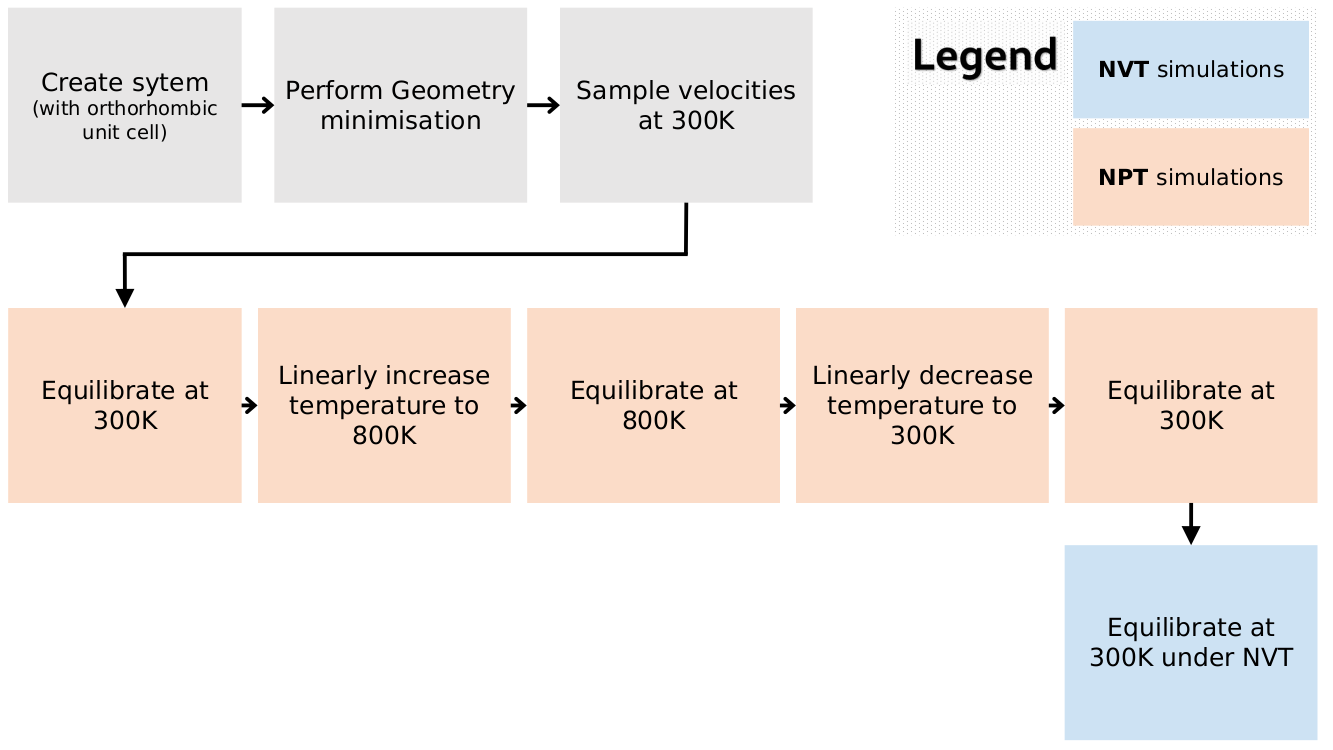
\includegraphics[width=\textwidth]{./img/FlowCharts/MeltQuench.png}
	\caption{\label{fig:meltQuenchFlowChart}The melt-quench scheme used to create amorphous pentacene systems. Blue boxes indicate steps using an NPT ensemble, orange boxes indicate use of a NVT ensemble.}
\end{figure}
\noindent In this procedure, the system was initialised with an individual pentacene molecule on a regular 3D grid using an orthorhombic unit cell. This was chosen to make analysis of the resulting structures easier than with the triclinic unit cell typically used to simulate pentacene crystals. The velocities were initially randomly sampled from a gaussian distribution and a Nose-Hoover thermostat and barostat was used to control the temperature and pressure. The Lammps molecular dynamics package was used \cite{LammpsMain, LammpsURL} and electrostatic interactions were handled with Lammps' particle-particle-particle-mesh ewald method \cite{LammpsPPPME}. RESP \cite{RESP} (restrained electrostatic potential) partial charges were parameterised using Gaussian 16 \cite{g16} with the B3-LYP level of theory and a G-311g(d) basis set. The use of partial charges was essential in the creation of the amorphous systems and will be discussed further in section \ref{sect:partial_charge_importance}. Finally, for inter and intra molecular interactions the general AMBER force-field \cite{GAFF} (GAFF) was applied. There doesn't seem to be one predominant forcefield to use in simulations of pentacene though parameters from GAFF have been used in a number of studies \cite{C0JM01577F, Yoneya2012, PentCrystallisation, MILLER201728, Wang2011, C6CP06436A, doi:10.1246/cl.180450}.
\\\\
Four different quenching times were used spanning 4 orders of magnitude: 0ns, 1ns, 10ns and 100ns. For the 0ns, 1ns and 10ns quenching simulations 3,000 molecules were simulated. In the 100ns quenched structure 3060 molecules were simulated. The initial structure for the 1ns and 10ns quenched structures were taken from a restart of the 0ns quenched simulation after the 800K equilibration step. The 0ns and 1ns quenched structure were carried out under 1 atmosphere of pressure in x, y and z. However, the 10ns quenching required a small increase to 5 atmospheres as the structure had a tendency to deform such that one of the cell vectors became either very large or very small. In the 100ns quenched structure I updated the barostat target pressure (before the phase transition) to account for similar deviations in simulation box dimensions.
\section{Structure of the quenched simulations}
A movie showing the full 100ns melt-quench simulation can be found here: \href{https://youtu.be/6IQcYErQHVs}{https://youtu.be/6IQcYErQHVs}. Still images of the final snapshot of each different quenching time are shown in figure \ref{fig:final_snapshots} below.
\\\\
\noindent We can see qualitatively that as we increase the quenching time from a) $\rightarrow$ d) the structure starts to look more ordered and crystal layers are starting to be formed. Looking longer at the structure we see that lower quench times tend to form small crystal clusters. In the 0ns quenched structure these clusters tend to be just $\sim$7-10 molecules in size. As we increase the quenching time to 1ns we see 1D channels of crystalline pentacene start to form throughout the structure, though the structure is still relatively disordered due to these channels being randomly oriented with respect to one another. As we increase the quenching time these crystal fragments become larger until in the 100ns quenched structure the whole system is comprised of just 2 crystals. The reason for this is, as we decrease the rate of cooling (increase quench time) we also decrease the rate of crystals being seeded. This allows any crystals that have formed to grow larger without being impeded by the growth of any other crystals. This can most clearly be seen in the animation of the \href{https://youtu.be/6IQcYErQHVs}{100ns melt quench simulation} linked above.

\begin{figure}[h]
	\includegraphics[width=\textwidth]{./img/DifferentQuenchTimes/AllTimes.png}
	\caption{\label{fig:final_snapshots}The final snapshot of each quenching simulation visualised in VMD \cite{VMD} and rendered with Tachyon \cite{Tachyon}. Snapshots are ordered by quenching time i.e. a) is the 0ns quench, b) is the 1ns quench and so on.}
\end{figure}
\noindent To quantify the change in the structure for the differently quenched structures 3 macroscopic properties can be plotted: the mass density, the angular distribution and the radial distribution function. These are discussed in the following sections.
\subsection{Mass Density}
The mass density of the 4 different quenching simulations can be seen below in figure \ref{fig:QuenchDensity}. This was calculated by dividing the total mass of the atoms in the system by the volume (product of cell vectors) of the simulation box. The first thing to notice in this graph is as we increase the quenching time we increase the density of the final sample. This is due to the molecules packing more efficiently in the crystal than in an amorphous structure. We also see very clearly in the plots the sudden increase in density associated with the phase transition from liquid to solid Pentacene. In the 1ns quench structure (quenched with the barostat set to 1 atmosphere) this occurs around Pentacene's experimental melting of 530.15K \cite{PentaceneMeltingPoint} providing confirmation of the choice of force-field. The 0ns, 1ns and 10ns runs were performed in a single 24 hour run. The 100ns quench was performed using many restarts, the discontinuities in the density for the 100ns structure come from these restarts. I don't believe they affect the final structure as these only occur while the system is in the liquid state.
\begin{figure}[H]
	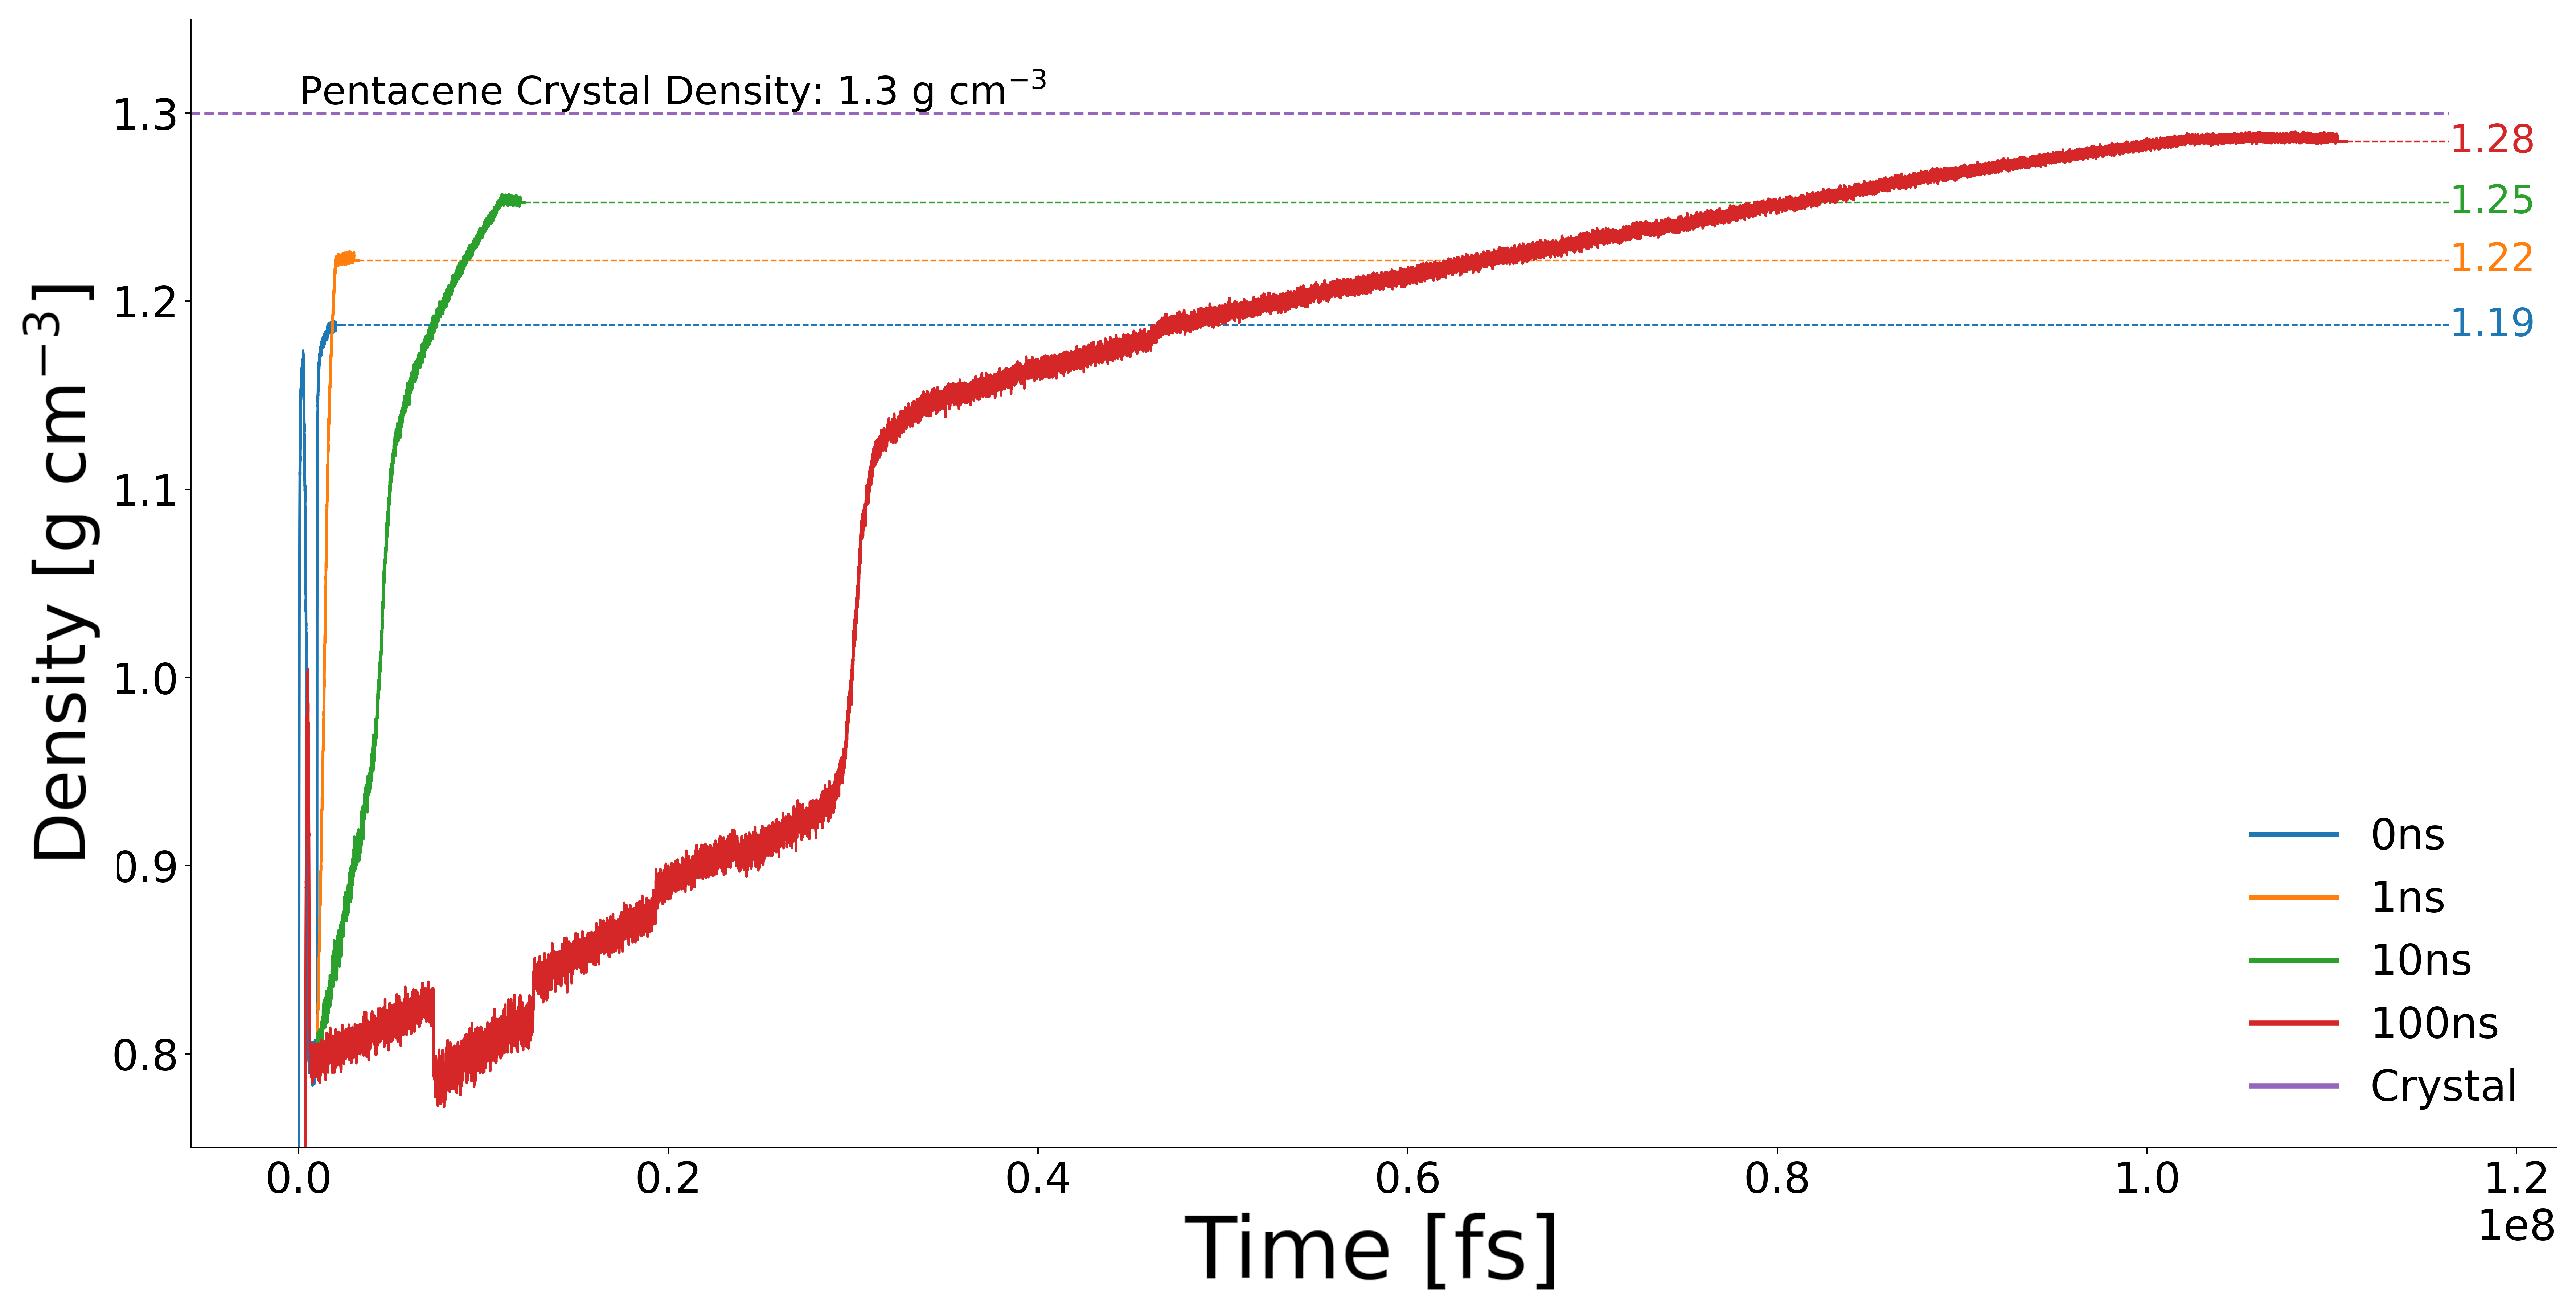
\includegraphics[width=\textwidth]{./img/DifferentQuenchTimes/Density.png}
	\caption{\label{fig:QuenchDensity}The time-evolution of the density of the differently quenched structures with annotations of the final density of each.}
\end{figure}

\subsection{Angular Distribution}
The angular distribution of the 4 quench times and a crystal structure before and after a short MD run is shown below in figure \ref{fig:ang_dist}. This was calculated by calculating the angle of an axis of each molecule with its nearest neighbours (20 $\AA$ center of mass cutoff was used). This data was then grouped into a histogram which is plotted below.
\begin{figure}[H]
	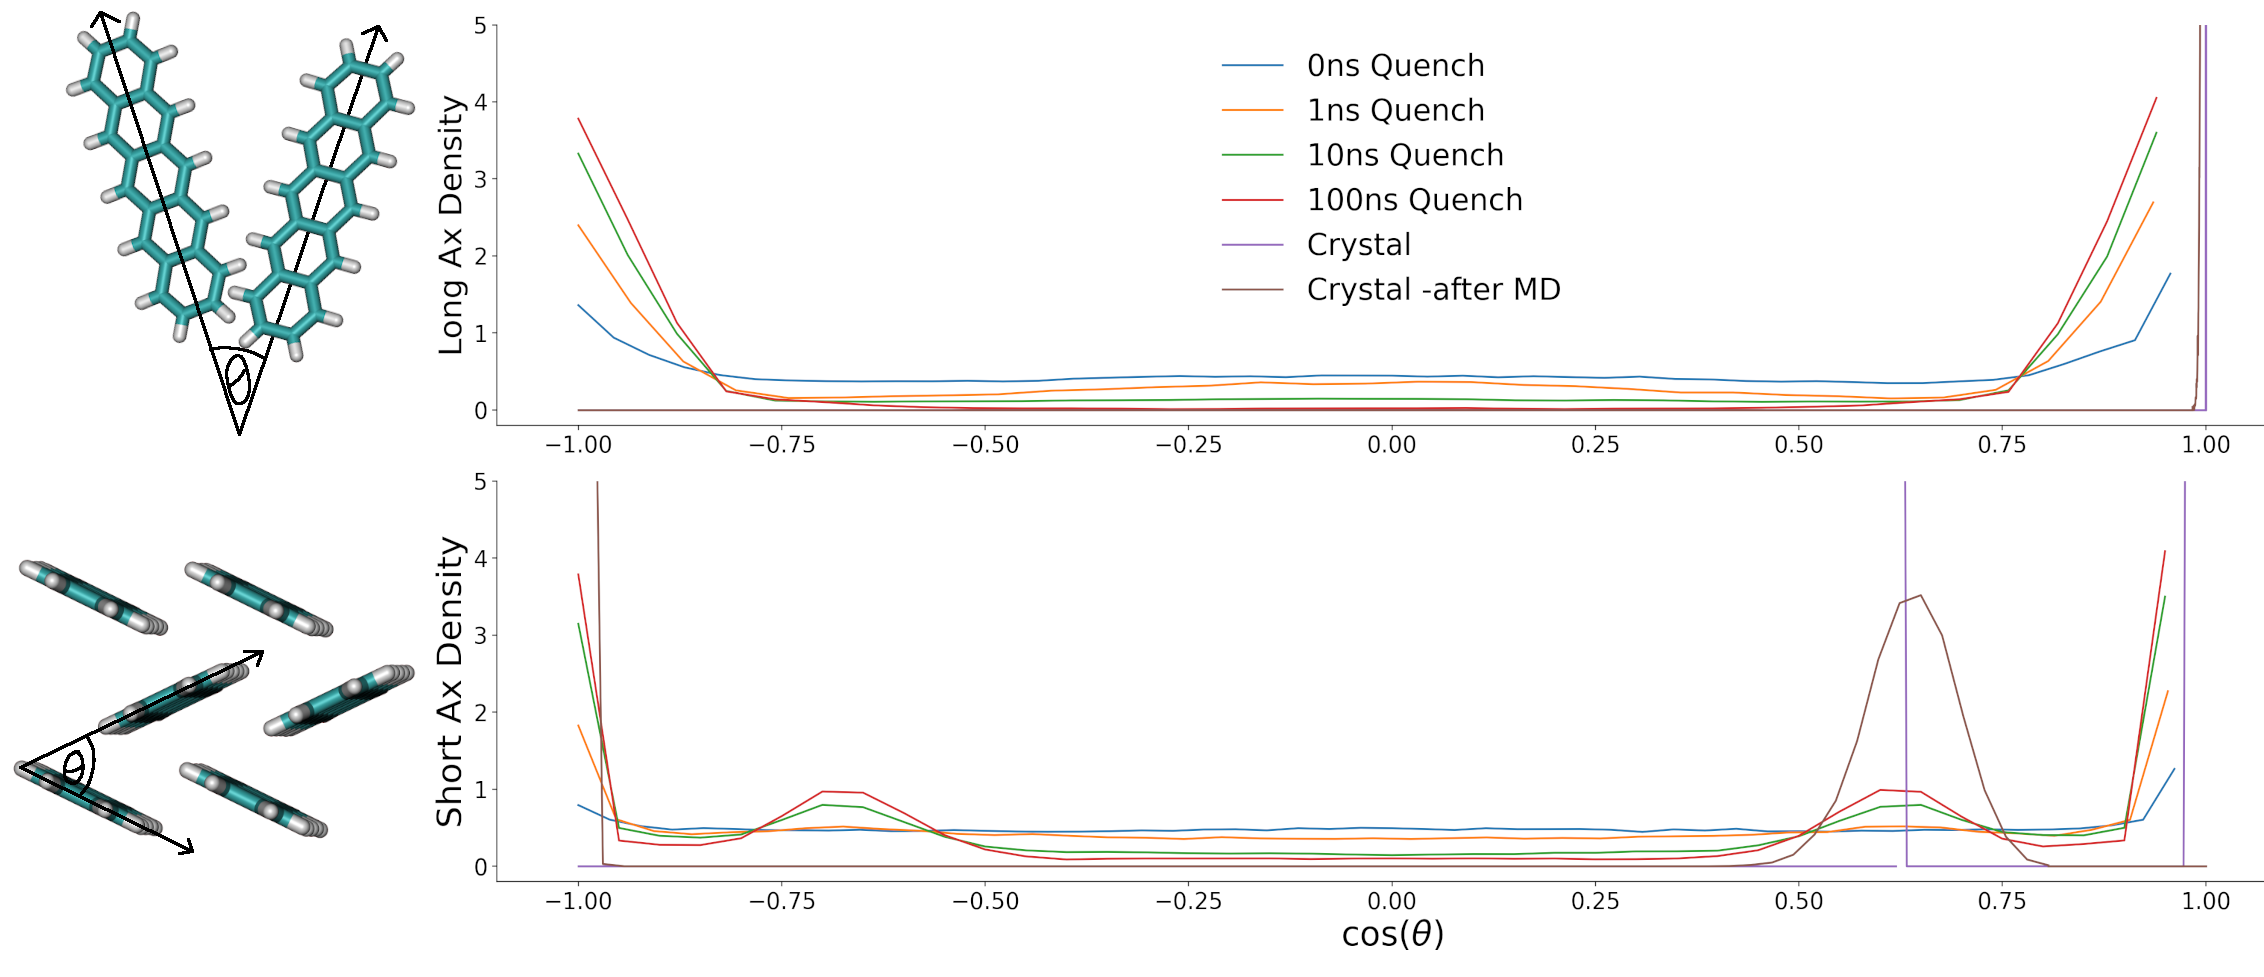
\includegraphics[width=\textwidth]{./img/DifferentQuenchTimes/AngularDist.png}
	\caption{\label{fig:ang_dist}The angular distribution for the 4 different quench times is shown above. The brown and purple lines are from a perfect crystal before and after a short MD run. The others are after the various melt-quench simulations. On the right is a schematic showing which angles are referenced in each plot.}
\end{figure}
In figure \ref{fig:ang_dist} we can see as the quenching time increases we start to notice an ever more prominent peak appear at either extreme of the x axis. This is because the molecules are aligning parallel with one another. The symmetry of the plot is an artefact of the melt stage of the simulation were each molecule was free to rotate randomly.
\\\\
If we now look at the short axis plot we can see that, again, as the quench time increases we start to see a more ordered structure start to form. This time the herringbone intersection angle between molecules (54.3$^{o}$ \cite{PentaceneAngle}) within the herringbone structure is retrieved. This is a result of using partial charges in the simulation -running the same simulations without partial charges results in an unrealistic face-to-face stacking. The brown and purple line show the same calculation run on a crystal of pentacene before and after MD. The purple line comes from an analysis of a repeated unit cell, hence we get 2 delta functions: one at 54.3$^{o}$ and one at 0$^{o}$. This structure was then equilibrated with electrostatics for 50ps and we start to see a broadening of the herringbone intersection angle and to a lesser extent (on the left side) a broadening of the angle between parallel pairs.
\subsection{Radial Distribution Function}
The radial distribution function for the 4 different quench times and the crystal before and after a short molecular dynamics equilibration is shown in figure \ref{fig:RDF}

\begin{figure}[h]
	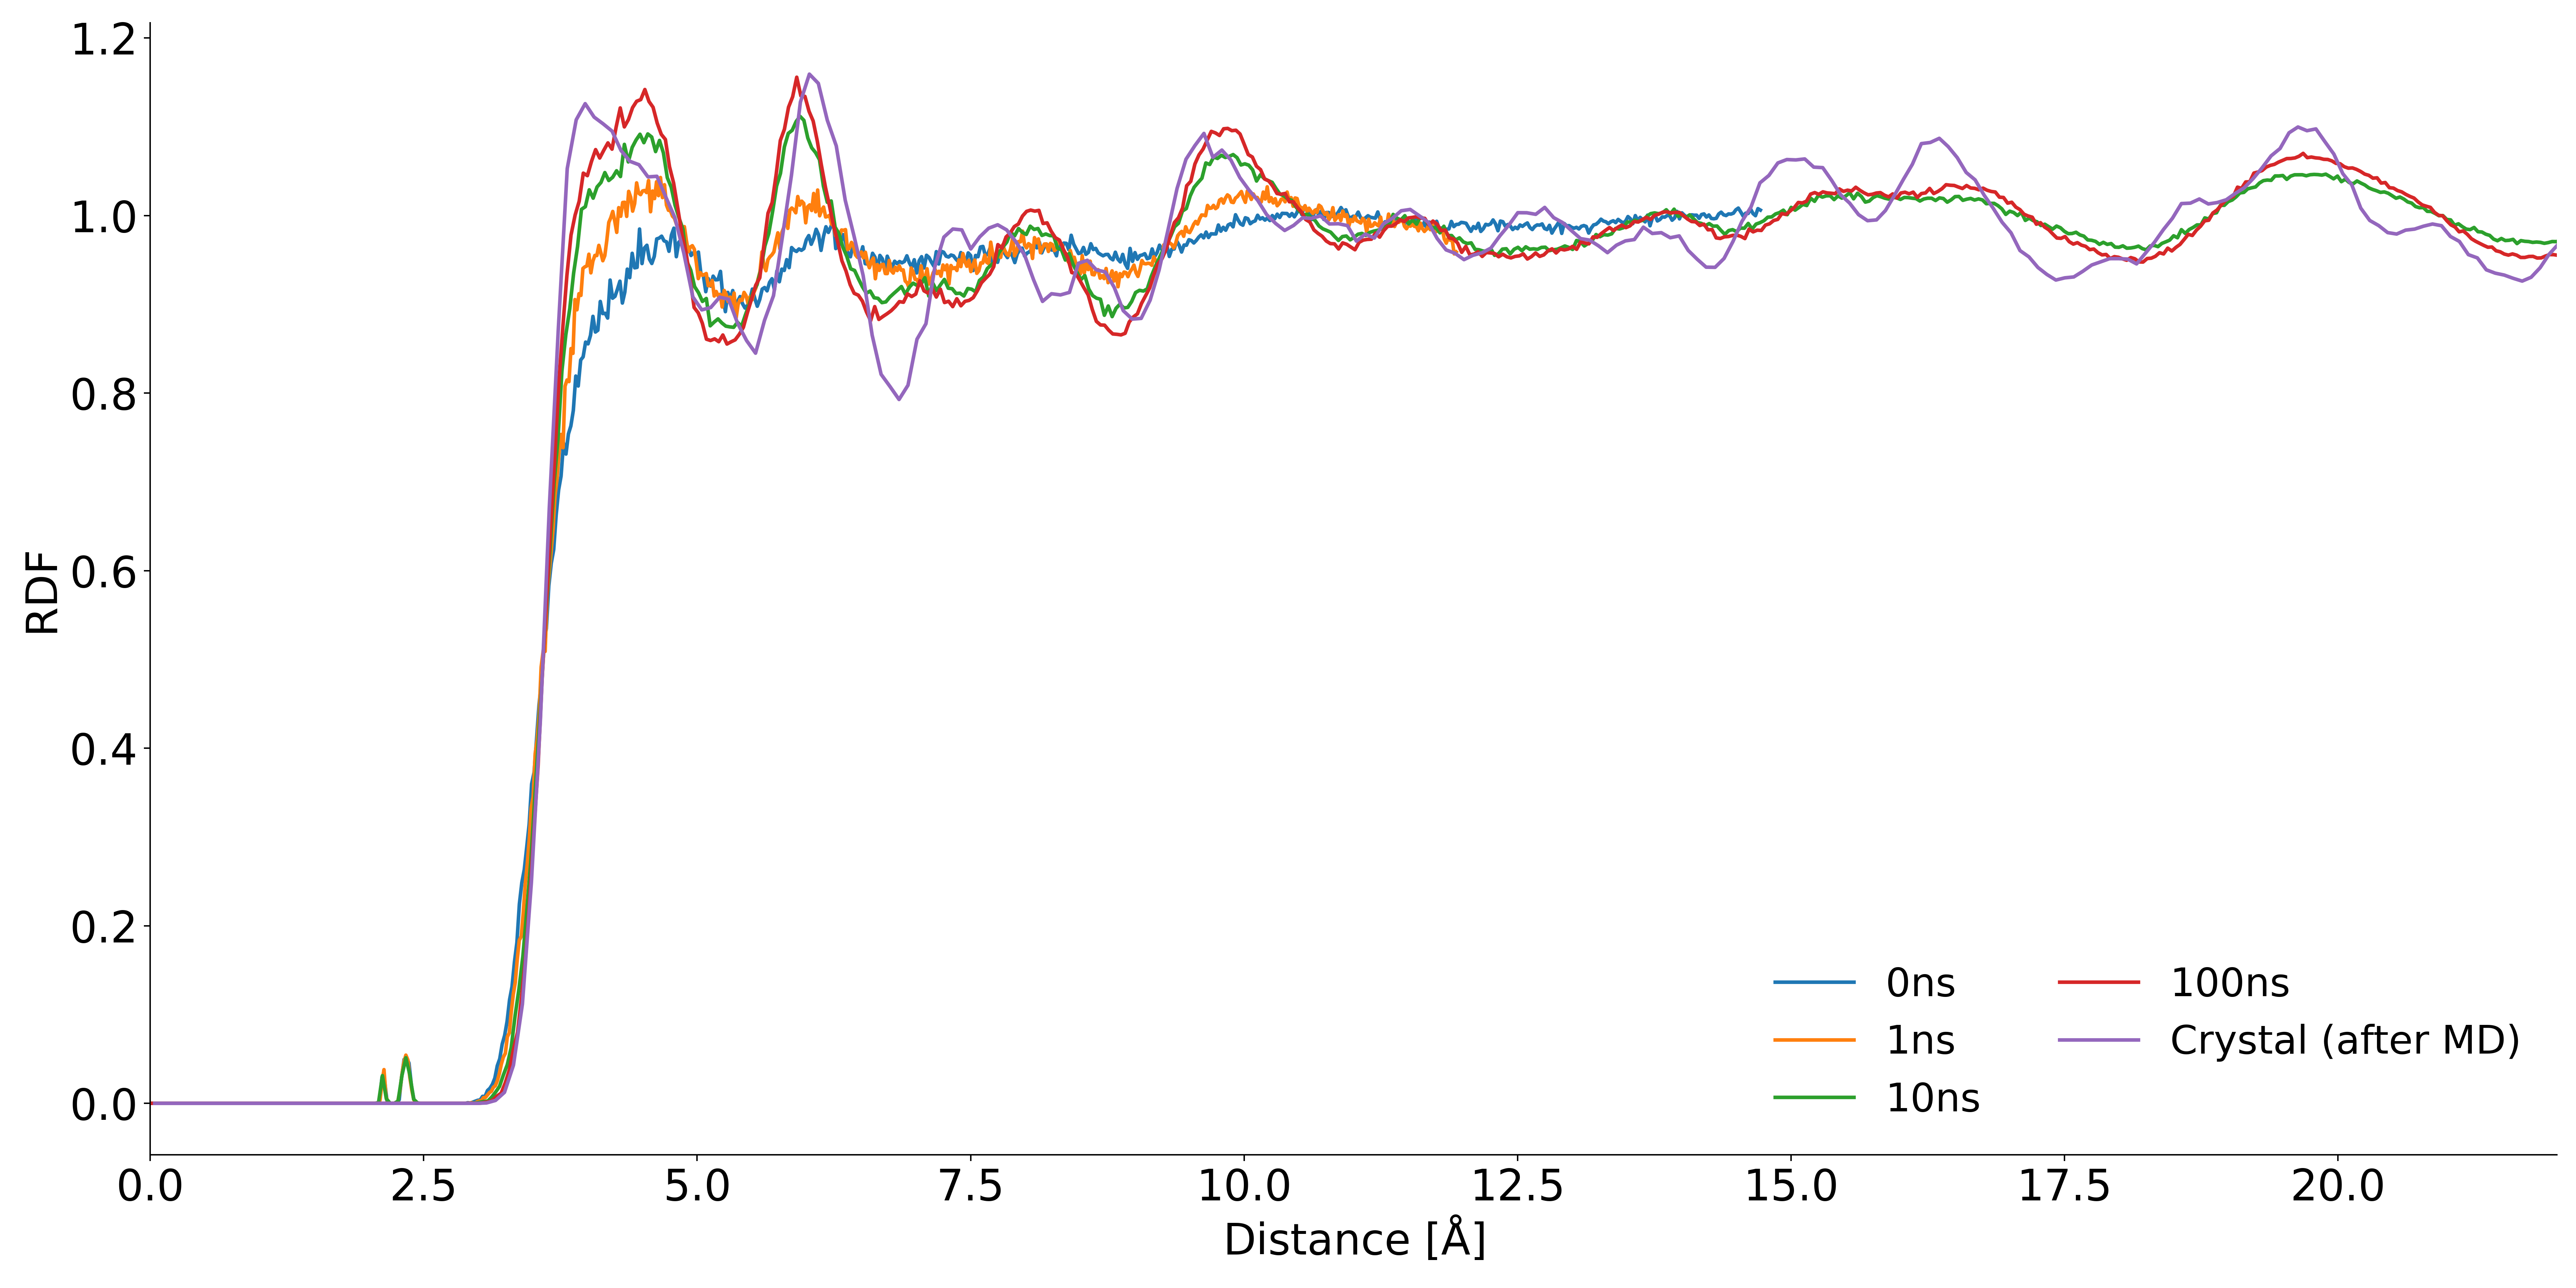
\includegraphics[width=\textwidth]{./img/DifferentQuenchTimes/RDF.png}
	\caption{\label{fig:RDF}The radial distribution function for 4 different quenching times and a crystal before and after 50ps of MD. The quenches (0, 1, 10 and 100ns) are shown in blue, orange, green and red respectively. The crystal data are shown in purple and brown.}
\end{figure}


\subsection{Molecular Dynamics without Partial Charges}
\label{sect:partial_charge_importance}

